\title{\textbf{F303 Intermediate Investments}}
\author{Lecture 22: Black-Scholes and Futures/Forwards \vspace{-1cm}}
\date{}
\frame[plain]{\titlepage}
\setcounter{framenumber}{0}

\pgfmathdeclarefunction{gauss}{2}{%
  \pgfmathparse{1/(#2*sqrt(2*pi))*exp(-((x-#1)^2)/(2*#2^2))}%
}



%%%%%%%%%%%%%%%%%%  SLIDE  %%%%%%%%%%%%%%%%%%
\frame{\frametitle{\large{\textbf{Goals for Today}}}
\begin{itemize}
\item Finish problem from last lecture

\item The basics of Futures Contracts

\item Mechanics of trading in futures markets

\item Futures market strategies

\item Determination of futures prices

\item Forward versus futures pricing
\end{itemize}
}

\frame{\frametitle{\large{\textbf{Review of Black-Scholes Formula}}} 
The price of a call and put option can be computed as follows:
\baa
C&=&S\times N(d1)-Ke^{-rT}\times N(d2)\\
P&=&Ke^{-rT}\times N(-d2)-S\times N(-d1)
\eaa
where $d_1$ and $d_2$ are defined as:
\baa
d_1&=&\frac{ln(S/K)+(r+\sigma^2/2)T}{\sigma \sqrt{T}}\\
d_2&=&d1-\sigma \sqrt{T}
\eaa
\begin{itemize}
\item $T$ is the time to maturity in years
\item $K$ is the strike price
\item $\sigma$ is the volatility of the stock
\item $r$ is the risk free rate
\end{itemize}
}




\frame{\frametitle{\large{\textbf{Problem 2}}} 

Assume that you hold the following portfolio of European options on the same stock:
\begin{itemize}
\item Long on a put with strike price of \$30;
\item Long on one call with strike price of \$30;
\item Short on two call with strike price of \$40;
\item Long a call option with strike price of \$50.
\end{itemize}
All options expire in 3 months. Assume that the stock price today is \$39 and that the stock volatility is 24\%. The continuously compounded risk-free interest rate is 5\%. Finally, assume that the Black-Scholes framework holds. 
}

\frame[t]{\frametitle{\large{\textbf{Problem 2}}} 
a) Compute the price of your portfolio.
}

\frame[t]{\frametitle{\large{\textbf{Problem 2}}} 
a) Compute the price of your portfolio.

\color{red}
Using the Black-scholes formula you can get the prices for the options. Here are the intermediate steps for the put with strike price of 30:
\baa
d_1&=&\frac{ln(S/K)+(r+\sigma^2/2)T}{\sigma \sqrt{T}}\\
&=&\frac{ln(39/30)+(0.05+0.24^2/2)0.25}{0.24 \sqrt{0.25}}\\
&=&2.3505\\
d_2&=&d1-\sigma \sqrt{T}=2.3505-0.24\sqrt{0.25}=2.2305\\
\eaa
}

\frame[t]{\frametitle{\large{\textbf{Problem 2}}} 
\color{red}
\begin{itemize}
\color{red}
\item Price of put @ 30 = 0.0153
\item Price of call @ 30 = 9.3880
\item Price of call @ 40 = 1.6371
\item Price of call @ 50 = 0.0488
\end{itemize}
The price of the portfolio is equal to $0.0153+9.3880-2\times 1.6371 + 0.0488=\$6.1779$
}

\frame[t]{\frametitle{\large{\textbf{Problem 2}}} 
b) Draw the \ul{profit} diagram for the portfolio specified above;
}

\frame[t]{\frametitle{\large{\textbf{Problem 2}}} 
b) Draw the \ul{profit} diagram for the portfolio specified above;
\begin{center}
\itemncludegraphics[scale=0.3]{./p1_b.jpg}
\end{center}

}


\frame[t]{\frametitle{\large{\textbf{Problem 2}}} 
c) Show that the put-call parity holds for the call and put option with strike price of \$30.

}

\frame[t]{\frametitle{\large{\textbf{Problem 2}}} 
c) Show that the put-call parity holds for the call and put option with strike price of \$30.
\color{red}
\textbf{Note:} I used continuous compounding in this solution. If you use discrete compounding, you will find that the put-call parity will not hold, which means that there is an arbitrage in this markets. 

\color{red}
\v

The price of the bond with face value of \$30 that expires in 4 months, using the interested rate given above, is:
\baa
B&=&=\$30\times e^{-0.05\times0.25}=29.6273
\eaa
The put-call parity states that:
\baa
P+S&=&C+B\\
\eaa
}
\frame[t]{\frametitle{\large{\textbf{Problem 2}}} 
\color{red}
Let's compute each part given the information from the previous part, and confirm that the equality holds.
\baa
P+S&=&0.0153+39=39.0153\\
C+B&=&9.3880+29.6273=39.0153
\eaa
The prices are precisely the same.
\color{black}
}




\frame{\frametitle{\large{\textbf{Futures and Forwards}}}
\begin{itemize}
\item Futures and forward contracts in many ways similar to options. They specify purchase or sale of some underlying asset at some future date.

\item However, for futures or forward contracts, \ul{the holder has the obligation} to go through with the agreed-upon transaction. 

\item That is, if you buy a futures contract, \ul{you have the obligation to buy the underlying asset for the agreed upon price at the agreed upon time!}
\end{itemize}
}

\frame{\frametitle{\large{\textbf{Futures and Forwards}}}
\begin{itemize}
\item Consider the case of an oil production company.  How much will the price of oil be in the future, when they are ready to sell the oil they produced?  The revenue of this company depends on oil prices, which are extremely volatile!

\item On the other hand, consider a company that has to buy oil as one of the inputs in the production process (airline company). This company has a problem that mirrors that of the oil production company. 

\item \textbf{Can forwards and futures help these two firms?}
\end{itemize}
}

\frame{\frametitle{\large{\textbf{Futures and Forwards}}} 
\begin{itemize}
\item \textbf{Yes!}  The two parties can enter into an agreement today that specifies the price at which the oil producer sells the oil to the other company in the future. 

\item Such an agreement will reduce the source of risk for both parties!  The oil producer delivers oil at a price agreed upon now, regardless of the market price at the time when oil is produced. 

\item This requires that \ul{BOTH parties be willing to lock in the price to be paid or received for delivery of the commodity.} 

\item This can be achieved using futures or forwards, which are similar contracts.

\end{itemize}
}

\frame{\frametitle{\large{\textbf{Futures versus Forwards}}} 
\begin{center}
\bt{|c|}
\hline
Forwards \\
\hline
Private contract between two parties \\
Not standardized\\
Specified delivery date (usually)\\
Settled at end of contract  \\
Delivery or final cash settlement usually takes place\\
\hline
\et
\\

\bt{|c|c|}
\hline
 Futures \\
 \hline
 Traded on an exchange \\
 Standardized contract \\
  Range of delivery dates \\
 Settled daily \\
 Contract usually closed out prior to maturity\\
 \hline
\et
\end{center}
}


\frame{\frametitle{\large{\textbf{Futures versus Forwards}}} 
\begin{itemize}
\item Because forwards are private contracts but futures are exchange traded, an additional difference is initial cash flow (i.e.  the cost of entering into the position).
\item \ul{Forwards:} no money changes hands until contract expiration
\item \ul{Futures:} traders must post an initial margin to open the position (usually 5-15\% of the total value of the contract) 

\item Note that, unlike option contracts, futures don't have a premium (cost)!  The contract doesn't cost anything.  Margin must be posted to secure the position, and over time, your gains and losses are netted against that.

\end{itemize}
}

\frame{\frametitle{\large{\textbf{Futures Contracts}}} 
\begin{itemize}
\item The trader in the long position is said to ``buy'' a contract; the short-side trader ``sells'' a contract. 

\item At maturity:

\begin{itemize}
\item Profit to long = Spot price at maturity - Original futures price
\v
\item Profit to short = Original futures price - Spot price at maturity
\end{itemize}

\item The spot price is the actual market price of the commodity at the time of the delivery.
\end{itemize}
}


\frame{\frametitle{\large{\textbf{Types of Futures Contracts}}} 
\begin{itemize}
\item  Foreign Currencies

\item Agricultural Products

\item Metals and Energy

\item Interest Rate Futures

\item Equity Indexes

\end{itemize}
}

\frame{\frametitle{\large{\textbf{Examples of Futures Contracts}}} 
\begin{center}
\itemncludegraphics[scale=0.4]{./gold}
\end{center}
}

\frame{\frametitle{\large{\textbf{Examples of Futures Contracts}}} 
\begin{center}
\itemncludegraphics[scale=0.4]{./sp500}
\end{center}
}


\frame{\frametitle{\large{\textbf{Examples of Futures Contracts}}} 
\begin{center}
\itemncludegraphics[scale=0.4]{./euro}
\end{center}
}

\frame{\frametitle{\large{\textbf{Examples of Futures Contracts}}} 
\begin{center}
\itemncludegraphics[scale=0.4]{./orange}
\end{center}
}


\frame{\frametitle{\large{\textbf{Payoffs from Futures Contracts}}} 
\begin{center}
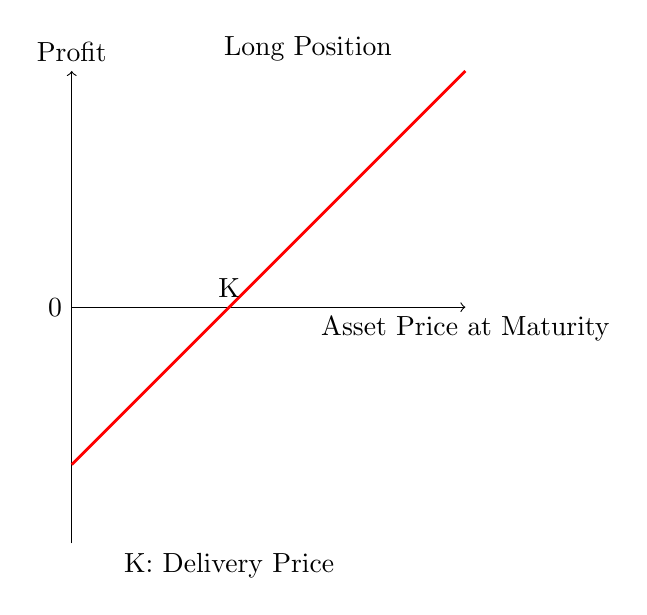
\begin{tikzpicture}
\draw (3,3) node[above] {Long Position};
\draw (0,3) node[above] {Profit};
\draw[->] (0,-3) -- (0,3);
\draw[->] (0,0) -- (5,0);
\draw[line width=1pt,red] (0, -2) -- (5, 3);
\draw (5,0) node[below] {Asset Price at Maturity};
\draw (2,0) node[above] {K};
\draw (0,0) node[left] {0};
\draw (2,-3) node[below] {K: Delivery Price};
\end{tikzpicture}
\end{center}
}


\frame{\frametitle{\large{\textbf{Payoffs from Futures Contracts}}} 
\begin{center}
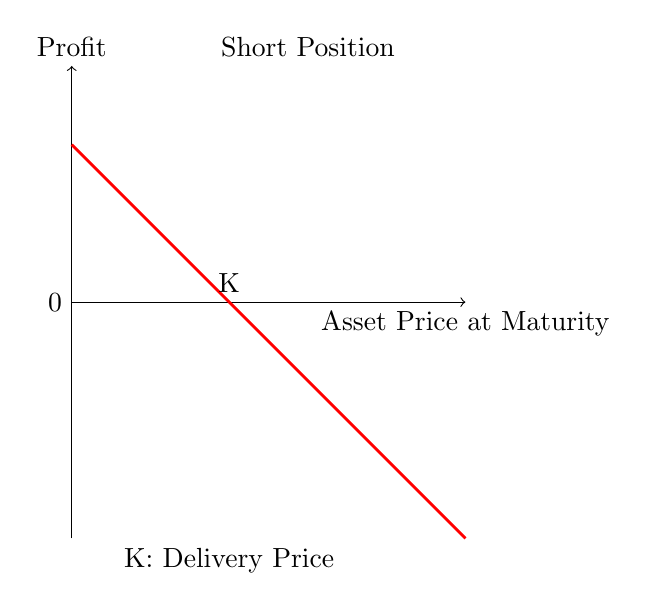
\begin{tikzpicture}
\draw (3,3) node[above] {Short Position};
\draw (0,3) node[above] {Profit};
\draw[->] (0,-3) -- (0,3);
\draw[->] (0,0) -- (5,0);
\draw[line width=1pt,red] (0, 2) -- (5, -3);
\draw (5,0) node[below] {Asset Price at Maturity};
\draw (2,0) node[above] {K};
\draw (0,0) node[left] {0};
\draw (2,-3) node[below] {K: Delivery Price};
\end{tikzpicture}
\end{center}
}



\frame{\frametitle{\large{\textbf{Marking to Market}}} 
\begin{itemize}
\item Traders of futures contracts must establish a \ul{margin account}. This account is a form of security consisting of cash so that the trader is able to satisfy the obligations of the futures contracts. Because both parties to a futures contract are exposed to losses, both must post margins. \ul{The initial margin is usually set between 5\% and 15\% of the total value of the futures contract.}

\item Let us say that you want to buy two June 2016 gold futures contracts. Suppose that the current futures price is \$1,660 per ounce; the contract size is 100 ounces. Hence the investor has contracted to buy a total of 200 ounces of gold.  Let us say that the broker has decided that the initial margin is \$3,000 per contract (\$6,000 in total). 

\end{itemize}
}


\frame{\frametitle{\large{\textbf{Marking to Market: An Example}}} 
\begin{itemize}
\item At the end of each trading day, the margin account is adjusted to reflect the investor's gain or loss. Let us assume that on December 15, the price drops from \$1,660 to \$1,657 per ounce. 

\item How much has the investor lost? 200 $\times$ \$3 = \$600. What is the new balance in the margin account? \$5,400

\item If your margin account falls below the maintenance margin level, you will receive a margin call.
\end{itemize}
}





\frame{\frametitle{\large{\textbf{Inherent Leverage}}} 
\begin{itemize}
\item Suppose initial margin for the oil contract is 10\%.  Current futures price is \$52.67, the contract size is 1,000 barrels/contract.

\item a) \ul{What is the margin in dollar terms?}
\baa
Margin=\$52.67 \times 1000 \times 10\%=\$ 5,267
\eaa
\item \ul{What is the underlying value of the position?}
\baa
Position=\$52.67\times 1000 = \$52,670
\eaa
\item Since you only pay a fraction of the overall value, \textbf{your returns are ``magnified'}' --- just like a leveraged position: \$2 increase oil prices (=3.797\% $\uparrow$) is a \$2,000 gain on the long position.
\baa
Return= 2,000/5,267=37.97\%!
\eaa
\baa
\eaa
\end{itemize}
}

